% ----------------------------------------------------------------------
%  Set the document class
% ----------------------------------------------------------------------
\documentclass[11pt,a4paper,twoside]{article}

% ----------------------------------------------------------------------
% Define external packages, language, margins, fonts and new commands
% ----------------------------------------------------------------------
%\input{preamble} 
\usepackage[utf8]{inputenc}   % <<<<< Linux
\usepackage[english]{babel} % <<<<< English
\usepackage{notoccite}
\usepackage[skip=0.5\baselineskip]{caption}
\hyphenation{GTKWave}
\usepackage{listings}
\usepackage[all]{nowidow}

\usepackage{float} %Nota: Adicionei esta package para poder usar o [H] nas figuras; ter em atenção que demasiados [H] consecutivos pode dar erro

%blind text
%\usepackage{lipsum}

\usepackage{graphicx}
\graphicspath{ {./} {../../figlib/} }
\def\FontLn{% 16 pt normal
  \usefont{T1}{phv}{m}{n}\fontsize{16pt}{16pt}\selectfont}
\def\FontLb{% 16 pt bold
  \usefont{T1}{phv}{b}{n}\fontsize{16pt}{16pt}\selectfont}
\def\FontMn{% 14 pt normal
  \usefont{T1}{phv}{m}{n}\fontsize{14pt}{14pt}\selectfont}
\def\FontMb{% 14 pt bold
  \usefont{T1}{phv}{b}{n}\fontsize{14pt}{14pt}\selectfont}
\def\FontSn{% 12 pt normal
  \usefont{T1}{phv}{m}{n}\fontsize{12pt}{12pt}\selectfont}

% Use Arial font as default
%
\renewcommand{\rmdefault}{phv}
\renewcommand{\sfdefault}{phv}
\usepackage{geometry}	
\geometry{verbose,tmargin=2.5cm,bmargin=2.5cm,lmargin=2.5cm,rmargin=2.5cm}

%\usepackage{setspace}
%\renewcommand{\baselinestretch}{1.5}

\usepackage[pdftex]{hyperref} % enhance documents that are to be
                              % output as HTML and PDF
\hypersetup{colorlinks,       % color text of links and anchors,
                              % eliminates borders around links
%            linkcolor=red,    % color for normal internal links
            linkcolor=black,  % color for normal internal links
            anchorcolor=black,% color for anchor text
%            citecolor=green,  % color for bibliographical citations
            citecolor=black,  % color for bibliographical citations
%            filecolor=magenta,% color for URLs which open local files
            filecolor=black,  % color for URLs which open local files
%            menucolor=red,    % color for Acrobat menu items
            menucolor=black,  % color for Acrobat menu items
%            pagecolor=red,    % color for links to other pages
            pagecolor=black,  % color for links to other pages
%            urlcolor=cyan,    % color for linked URLs
            urlcolor=black,   % color for linked URLs
	          bookmarks=true,         % create PDF bookmarks
	          bookmarksopen=false,    % don't expand bookmarks
	          bookmarksnumbered=true, % number bookmarks
	          pdftitle={report},
            pdfauthor={Alexandre Sequeira, Duarte Marques, João Chaves},
%            pdfsubject={Thesis Title},
%            pdfkeywords={Thesis Keywords},
            pdfstartview=FitV,
            pdfdisplaydoctitle=true}

\usepackage[numbers,sort&compress]{natbib} % <<<<< References in numbered list [1],[2],...
\usepackage{subcaption} 
\usepackage{mdframed}

%%%%%%%%%%%%%%%%%%%%%%%%%%%%%%%%%%%%%%%%%%%%%%%%%%%%%%%%%%%%%%%%%%%%%%%%
%     Begin Document                                                   %
%%%%%%%%%%%%%%%%%%%%%%%%%%%%%%%%%%%%%%%%%%%%%%%%%%%%%%%%%%%%%%%%%%%%%%%%


\begin{document}

% Set plain page style (no headers, footer with centered page number)
\pagestyle{plain}

% Set roman numbering (i,ii,...) before the start of chapters
%\pagenumbering{roman}

% ----------------------------------------------------------------------
%  Cover page
% ----------------------------------------------------------------------
\thispagestyle {empty}

% IST Logo - Signature A
% parameters: bb=llx lly urx ury (bounding box), width=h_length, height=v_length, angle=angle, scale=factor, clip=true/false, draft=true/false. 
\includegraphics[bb=9.5cm 11cm 0cm 0cm,scale=0.29]{IST_A_CMYK_POS}

\begin{center}

% Figure (Image or plot)
\vspace{1.0cm}
% height = 50 mm
%\includegraphics[height=50mm]{Figures/Airbus_A350.jpg}

% Title, author and degree
\vspace{1cm}
{\FontLb Circuit Theory and Electronics Fundamentals} \\ % <<<<< EDIT TITLE
\vspace{0.5cm}
{\FontSn Integrated Master in Engineering Physics, IST, University of Lisbon} \\
\vspace{0.5cm}
{\FontSn Lab 1: Circuit analysis methods} \\
\vspace{0.2cm}
{\FontSn Alexandre Sequeira(96503), Duarte Marques(96523), João Chaves(96540)} \\
\vspace{0.2cm}
{\FontSn March 25, 2021} \\ % <<<<< EDIT DATE (corresponds to date of oral examination)
%
\end{center}



% ----------------------------------------------------------------------
% Dedication page (optional)
% ----------------------------------------------------------------------
%\input{dedication} 
%\cleardoublepage

% ----------------------------------------------------------------------
%  Acknowledgments (optional)
% ----------------------------------------------------------------------
%\input{acknowledgements}
%\cleardoublepage

% ----------------------------------------------------------------------
%  Abstract (both in English and Portuguese)
% ----------------------------------------------------------------------
%\input{resumo} 
%\cleardoublepage

%\input{abstract} 

% ----------------------------------------------------------------------
%  Table of contents, list of tables, list of figures and nomenclature
% ----------------------------------------------------------------------

% Table of contents
%
\tableofcontents

% List of tables
%\addcontentsline{toc}{section}{\listtablename}
%\listoftables
%\cleardoublepage 

% List of figures
%\addcontentsline{toc}{section}{\listfigurename}
%\listoffigures
%\cleardoublepage 

% Set arabic numbering (1,2,...) after preface
%
%\setcounter{page}{1}
%\pagenumbering{arabic}

% ----------------------------------------------------------------------
%  Body
% ----------------------------------------------------------------------

\section{Introduction} \label{sec:introduction}

In this laboratory assignment, a band pass filter (BPF) with an OP-AMP was implemented and studied. Using the circuit shown in Figure \ref{fig:CircuitDraw}, a theoretical analysis was made and its results were obtained by using the Octave math tool. Moreover, an Ngspice script was made in order to simulate this circuit. In both cases, the values of the central frequency, the input and output impedances at this frequency and the gain in the passband were determined. The plot of the frequency response has been obtained for both analyses, in which the values used for the resistances and capacitances shown in Figure \ref{fig:CircuitDraw} are presented in Table \ref{tab:chosen_values} of Section \ref{sec:analysis}. As seen below, designations have been assigned to each node in the circuit.
\par
As opposed to the previous laboratory assignments, it was also possible to test out this circuit presentially. Therefore, the circuit's gain was determined for different values of the components and these results will be shown in this report. It is worth noting that, even though the resistance $R_{2p}$ ended up not being considered for the theoretical and simulation analysis, it is still shown below, as it was used in the laboratory.

\begin{figure}[H] \centering
  \includegraphics[width=0.95\linewidth]{CircuitDraw.pdf}
  \caption{Circuit to be analysed in this laboratory assignment.}
  \label{fig:CircuitDraw}
\end{figure}


\section{Theoretical Analysis}

The values of the resistances $R_1$ and $R_2$ and of the capacitance $C$ have been chosen arbitrarily, in order to obtain the best results and the best merit $M$ possible. These values are shown below.

\begin{table}[H]
  \centering
  \begin{tabular}{|c|c|}
    \hline    
    {\bf Name} & {\bf Value} \\ \hline
    \input{../mat/ChosenValues.tex}
  \end{tabular}
  \caption{Values used for the resistances $R_1$ and $R_2$ and for the capacitance $C$.}
  \label{tab:ChosenValues}
\end{table}

Assuming that the transformers' wires are coiled according to the conventional way, that is, in order to generate a downwards current through the left transformer (transformer 1) and an upwards current through transformer 2 (on the right), we have that $v_{t1}$=$n$ $v_{t2}$, with $n$ being the number of turns in transformer 1, $v_{t1}$ the AC signal in transformer 1 and $v_{t2}$ in transformer 2. Because the objective is to obtain a DC voltage of $12$V in the output, a sinusoidal signal of amplitude $50$V was used for transformer 2, thus the value of $n$ was given by $n=\frac{V_{t1}}{V_{t2}}=\frac{230}{5}$, with $V_{t1}=230$V and $V_{t2}=50$V being the amplitudes of the sinusoidal signals in the respective transformers.
\par
Because of the 4 diodes in the full-wave bridge rectifier circuit, the voltage through the resistance $R_1$ is given by

\begin{equation} \label{eq:rectified_voltage}
  v_{O_{rectified}}(t)=|v_{t2}|
\end{equation}

Where an ideal diode model has been considered. Now, the capacitor is used to keep the voltage approximately constant and close to $12$V. As was learnt in class, the time it takes for the diode circuit to go OFF and for the capacitor to start discharging through the resistance $R_1$ is given by

\begin{equation} \label{eq:toff}
  t_{OFF}=\frac{1}{\omega}atan\left(\frac{1}{\omega R_1C}\right)
\end{equation}

Where $\omega=2\pi f$, with $f=50$Hz as shown in Figure \ref{fig:CircuitDraw}. After $t_{OFF}$, the voltage in the output of the envelope detector is not $v_{O_{rectified}}(t)$, but

\begin{equation} \label{eq:exponential_voltage}
  v_{O_{envelope}}(t)=V_{t2}cos(\omega t_{OFF})e^{-\frac{t-t_{OFF}}{R_1C}}
\end{equation}

When the time instant $t_{ON}$ is reached, the voltage is again given by equation \ref{eq:rectified_voltage}. To determine $t_{ON}$, the following non-linear equation must be solved:

\begin{equation} \label{eq:non_linear_equation_tON}
  V_{t2}cos(\omega t_{ON})=V_{t2}cos(\omega t_{OFF})e^{-\frac{t_{ON}-t_{OFF}}{R_1 C}}
\end{equation}

The value of $t_{ON}$ was obtained by Octave and by using Newton-Raphson's iterative nethod. The following values were obtained:

\begin{table}[H]
  \centering
  \begin{tabular}{|c|c|}
    \hline    
    {\bf Name} & {\bf Value} \\ \hline
    \input{../mat/tOFF_tON.tex}
  \end{tabular}
  \caption{Values obtained for $t_{ON}$ and $t_{OFF}$.}
  \label{tab:tON_tOFF}
\end{table}

Using this information, the rectified and final voltage out of the envelope detector were plotted together, as shown below.


\begin{figure}[H] \centering
  \includegraphics[width=0.7\linewidth]{envelope.eps}
  \caption{Voltages in the envelope detector and voltage regulator circuits.}
  \label{fig:envelope_regulator_voltages}
\end{figure}

\begin{figure}[H] \centering
  \includegraphics[width=0.7\linewidth]{variations.eps}
  \caption{Deviation of final voltage regulator voltage from $12$ $V$.}
  \label{fig:voltage_variation}
\end{figure}

\begin{table}[H]
  \centering
  \begin{tabular}{|c|c|}
    \hline    
    {\bf Name} & {\bf Value} \\ \hline
    \input{../mat/Merit.tex}
  \end{tabular}
  \caption{Cost and merit obtained from the Theoretical Analysis.}
  \label{tab:Cost_Merit}
\end{table}


\section{Simulation Analysis}
\label{sec:simulation}

\subsection{Exercise 1}

Table~\ref{tab:Exercise1Simulation} shows the simulated operating point results for the circuit presented in Figure \ref{fig:CircuitDraw}. Again, currents designated below as $I_i$ refer to the currents passing through the respective resistances, $R_i$.

\begin{table}[H]
  \centering
  \begin{tabular}{|c|c|}
    \hline    
    {\bf Designation} & {\bf Value [A or V]} \\ \hline
    \input{../sim/Exercise1_tab.tex}
  \end{tabular}
  \caption{Operating point analysis table. Currents $I_i$ are in amperes; voltages $V_i$ are in volts.}
  \label{tab:Exercise1Simulation}
\end{table}

Comparing the theoretical analysis results presented in Table \ref{tab:Exercise1Theoretical} and the results in Table \ref{tab:Exercise1Simulation}, we can notice almost no differences. This was to be expected, since the circuit has no time dependency - meaning it's equal at any point in time. There is only a small difference between the two values of $I_c$, although it is negligible.\par
Now we ca approach the second point of our simulation where we see how the system behaves when $v_s(0)=0$ and the capacitor is replaced by a voltage souce $V_X$=V(6)-V(8), where the voltages are taken from \ref{tab:Exercise1Simulation}.

\begin{table}[H]
  \centering
  \begin{tabular}{|c|c|}
    \hline    
    {\bf Designation} & {\bf Value [A or V]} \\ \hline
    \input{../sim/Exercise2_tab.tex}
  \end{tabular}
  \caption{Operating point analysis table. Currents $I_i$ are in amperes; voltages $V_i$ are in volts.}
  \label{tab:Exercise2Simulation}
\end{table}

\subsection{Transient analisis}

Now we do a transient analisis of the values.

\begin{figure}[h] \centering
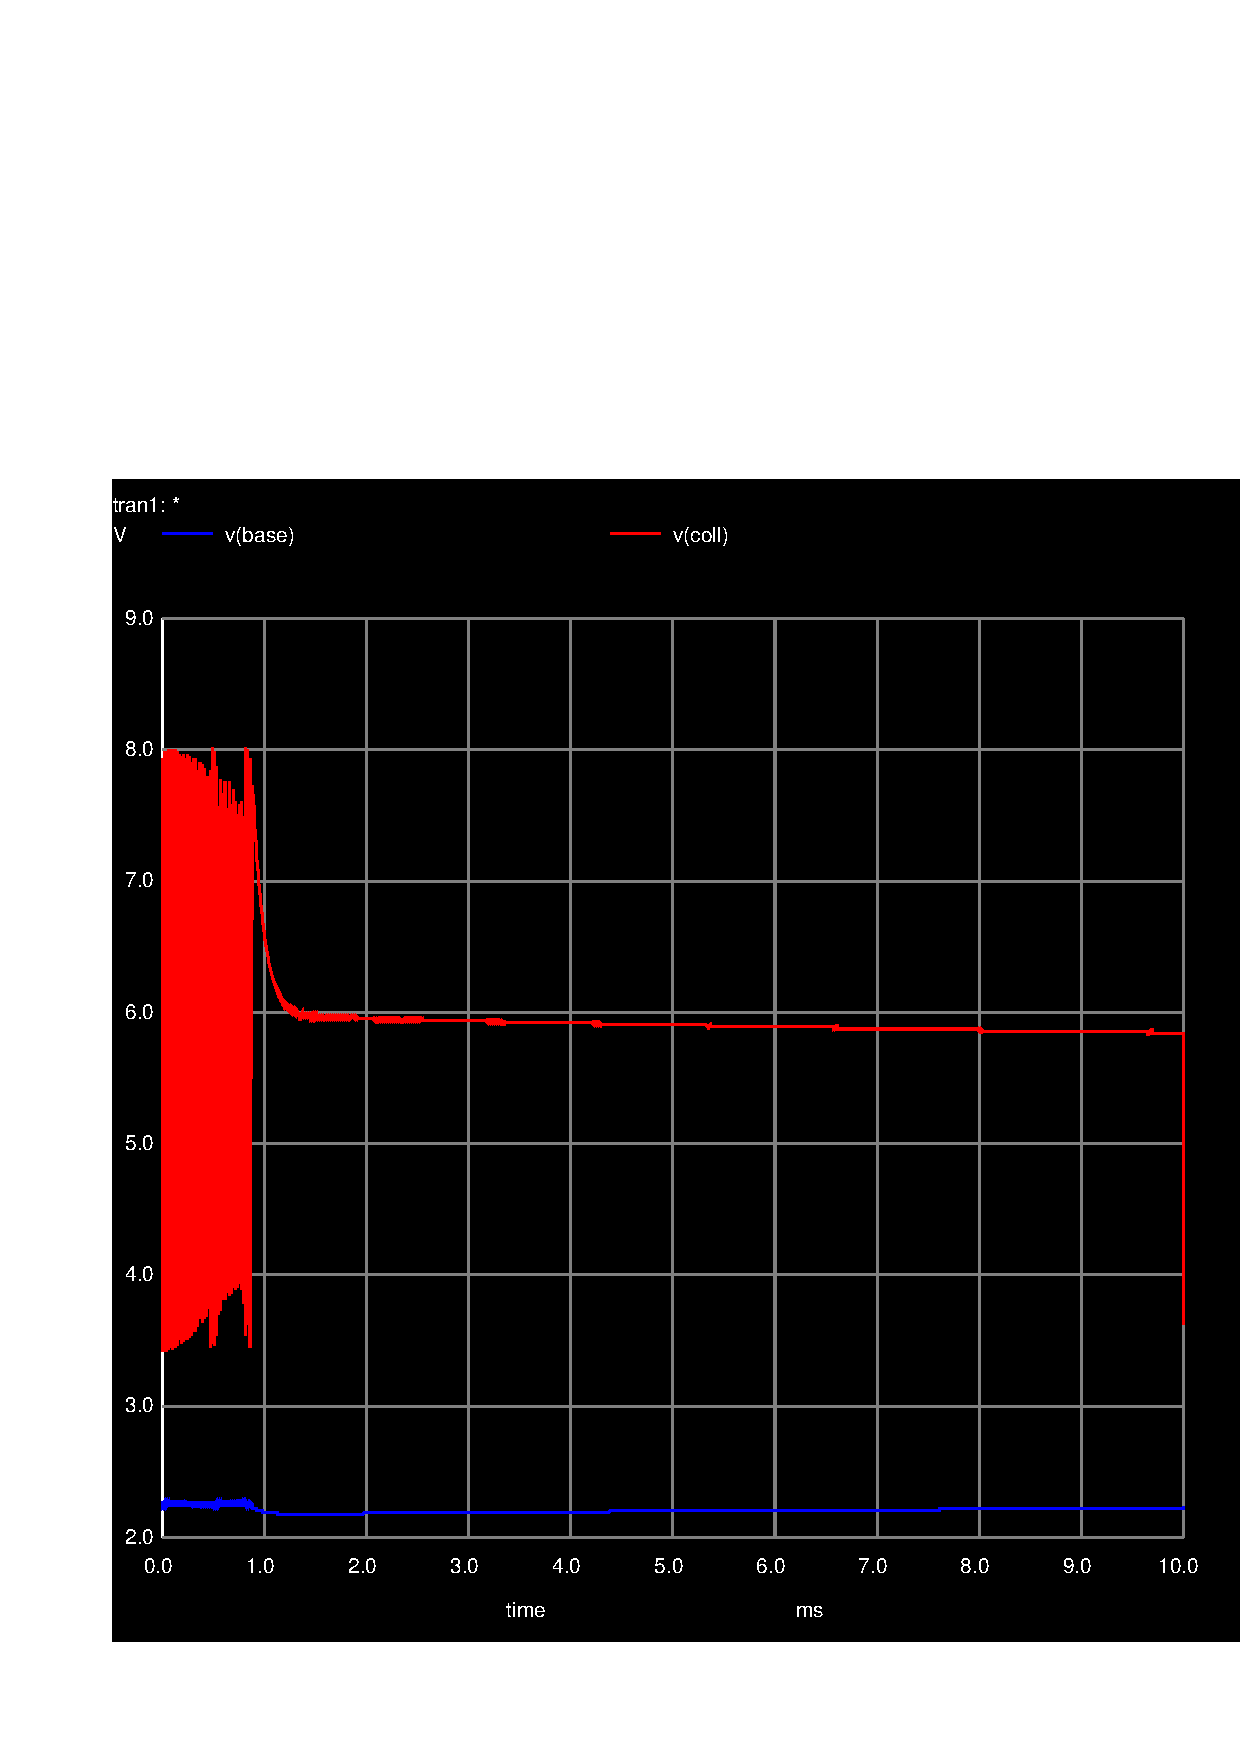
\includegraphics[width=0.8\linewidth]{../sim/trans.pdf}
\caption{Natural response.}
\label{fig:forced}
\end{figure}


\begin{figure}[h] \centering
\includegraphics[width=0.8\linewidth]{../sim/trans1.pdf}
\caption{Forced sinusoidal response and stimulus.}
\label{fig:forced}
\end{figure}


\section{Conclusion}

In this laboratory assignment, the objective of 

%\cleardoublepage

% ----------------------------------------------------------------------
%  Bibliography
% ----------------------------------------------------------------------
%\addcontentsline{toc}{section}{\bibname}
%\bibliographystyle{abbrvunsrtnat} % <<<<< SELECT IF USING REFERENCES BY NUMBER (CITATION ORDER)
%\bibliography{../../../BIBfile.bib}

% ----------------------------------------------------------------------
\end{document}
% ----------------------------------------------------------------------

